\documentclass[11pt, a4paper]{article}

% --- 基础宏包配置 ---
\usepackage[utf8]{inputenc}
\usepackage{ctex} % 支持中文输出
\usepackage{geometry} % 调整页边距
\usepackage{graphicx} % 插入图片必备
\usepackage{caption}  % 美化图题（可选，期刊论文推荐）
\usepackage{float}
\usepackage{booktabs}
\usepackage{xcolor}
\usepackage{graphicx}
\geometry{top=2.5cm, bottom=2.5cm, left=2.5cm, right=2.5cm}

\usepackage{amsmath, amssymb} % 数学公式
\usepackage{graphicx} % 插入图片
\usepackage{booktabs} % 三线表
\usepackage{cite} % 参考文献
\usepackage{enumitem}

% --- 【新增】超链接与PDF书签配置 ---
\usepackage{hyperref} 
\hypersetup{
	colorlinks=true,      % 开启彩色链接（打印时若不需要可设为false）
	linkcolor=blue,       % 内部链接（如目录、公式、图表跳转）为蓝色
	citecolor=blue,       % 文献引用（如 [1]）为蓝色
	urlcolor=magenta,     % 外部网页链接为洋红色
	pdfstartview={FitH}   % 打开PDF时自动水平适应页面宽度
}

% --- 标题与个人信息 ---
\title{\textbf{基于论文复现Transformer quantum state: A multipurpose model for
		quantum many-body problems}}
\author{完成人：李想 }
\date{\today} % 自动显示当前日期

\begin{document}
	
	\maketitle
	
	\hrule
	\vspace{1em}
	
	% --- 【新增】自动目录部分 ---
	% 提示：如果报告只有 1-2 页，可以把这两行删掉；若超过 3 页，建议保留。
	\tableofcontents
	\newpage % 目录生成后强制换页，让正文结构更整洁
	
	% --- 1. 实验目的 ---
	\section{实验目的 (Objectives)}
	对论文Transformer quantum state: A multipurpose model for
	quantum many-body problems尝试复现工作。
	\begin{itemize}
		\item 横场伊辛模型的精确对角化基准测试。
		\item 蒙特卡洛采样收敛性测试
		\item 未经过优化的RBM初始能量计算与评估
		\item RBM-变分蒙特卡洛优化
	\end{itemize}
	
	% --- 2. 实验方案/方法 ---
	\section{步骤一:横场伊辛模型的精确对角化基准测试}
	为了验证横场伊辛哈密顿量的代码实现，我们首先对有限尺寸系统进行了精确对角化分析。在临界点（$J=1, h=1$）下，我们计算了不同系统尺寸的基态能量密度 $e_0(N)=E_0(N)/N$。
	% 单张图片环境
	\begin{figure}[H] % [H]强制固定在当前文字下方，不会乱跑
		\centering
		% 宽度占页面文本80%，文件名替换成你results里的图片
		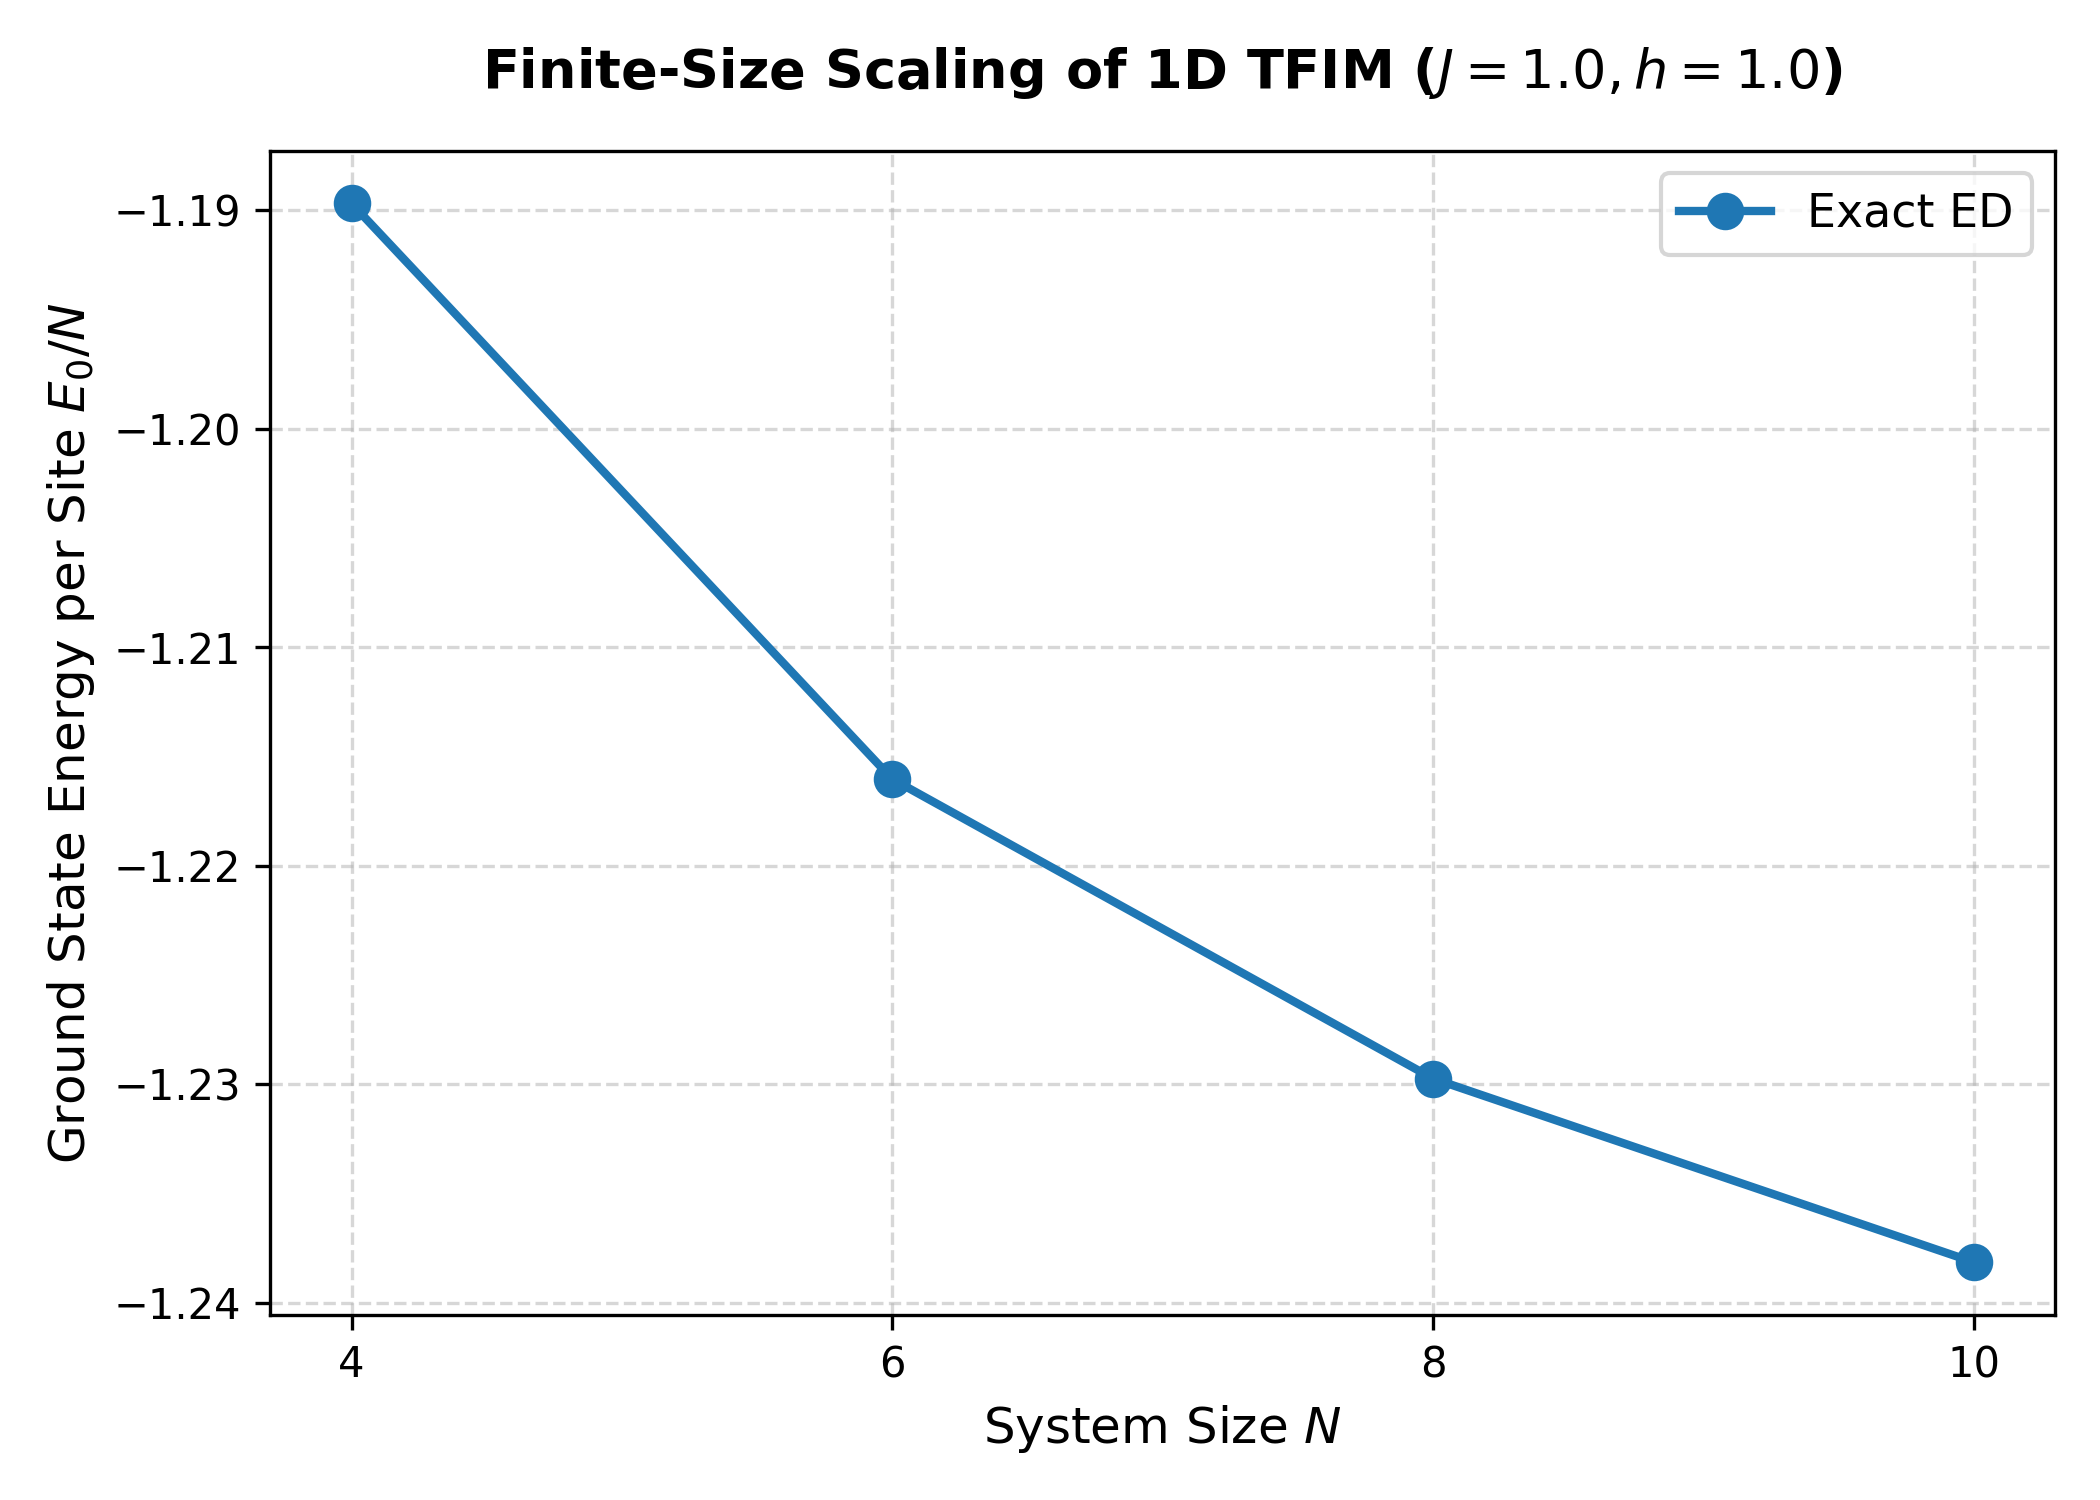
\includegraphics[width=0.8\textwidth]{../results/ising_fss_plot.png}
		\caption{临界点$J=h=1$下不同系统尺寸$N$对应的基态能量密度曲线}
		\label{图一}
	\end{figure}
	如图 1 所示，随着系统尺寸的增加，能量密度逐渐降低并趋于一个稳定值，这表明结果正在向热力学极限收敛。较小尺寸 $N$ 所带来的偏差源于有限尺寸效应，此时边界贡献变得十分显著：
	\begin{equation}
		E_0(N)=Ne_\infty+E_{\text{boundary}}
	\end{equation}
	该计算提供了一个可靠的基准，用于在后续阶段评估变分神经网络量子态的性能。
	
	\begin{table}[htbp]
		\centering
		\caption{实验核心参数设置}
		\label{tab:parameters}
		\begin{tabular}{lcc}
			\toprule
			参数名称 & 设定值 & 备注 \\
			\midrule
			学习率 (Learning Rate) & $0.001$ & 沿用上周最佳配置 \\
			批次大小 (Batch Size) & 64 & - \\
			迭代次数 (Epochs) & 100 & 观察是否过拟合 \\
			\bottomrule
		\end{tabular}
	\end{table}
	
	% --- 3. 实验结果与分析 ---
	\section{蒙特卡洛采样收敛性测试}
	为了评估 VMC（变分蒙特卡洛）能量估计器的统计可靠性，我们研究了估计能量对蒙特卡洛样本数量的依赖关系。
	对于一个固定的试验波函数，变分能量的估计公式为：
	\begin{equation}
		E_{VMC} = \frac{1}{N_s} \sum_{i=1}^{N_s} E_{loc}(s_i)
	\end{equation}
	其中 $N_s$ 代表蒙特卡洛样本的数量。
	\begin{figure}[H]
		\centering
		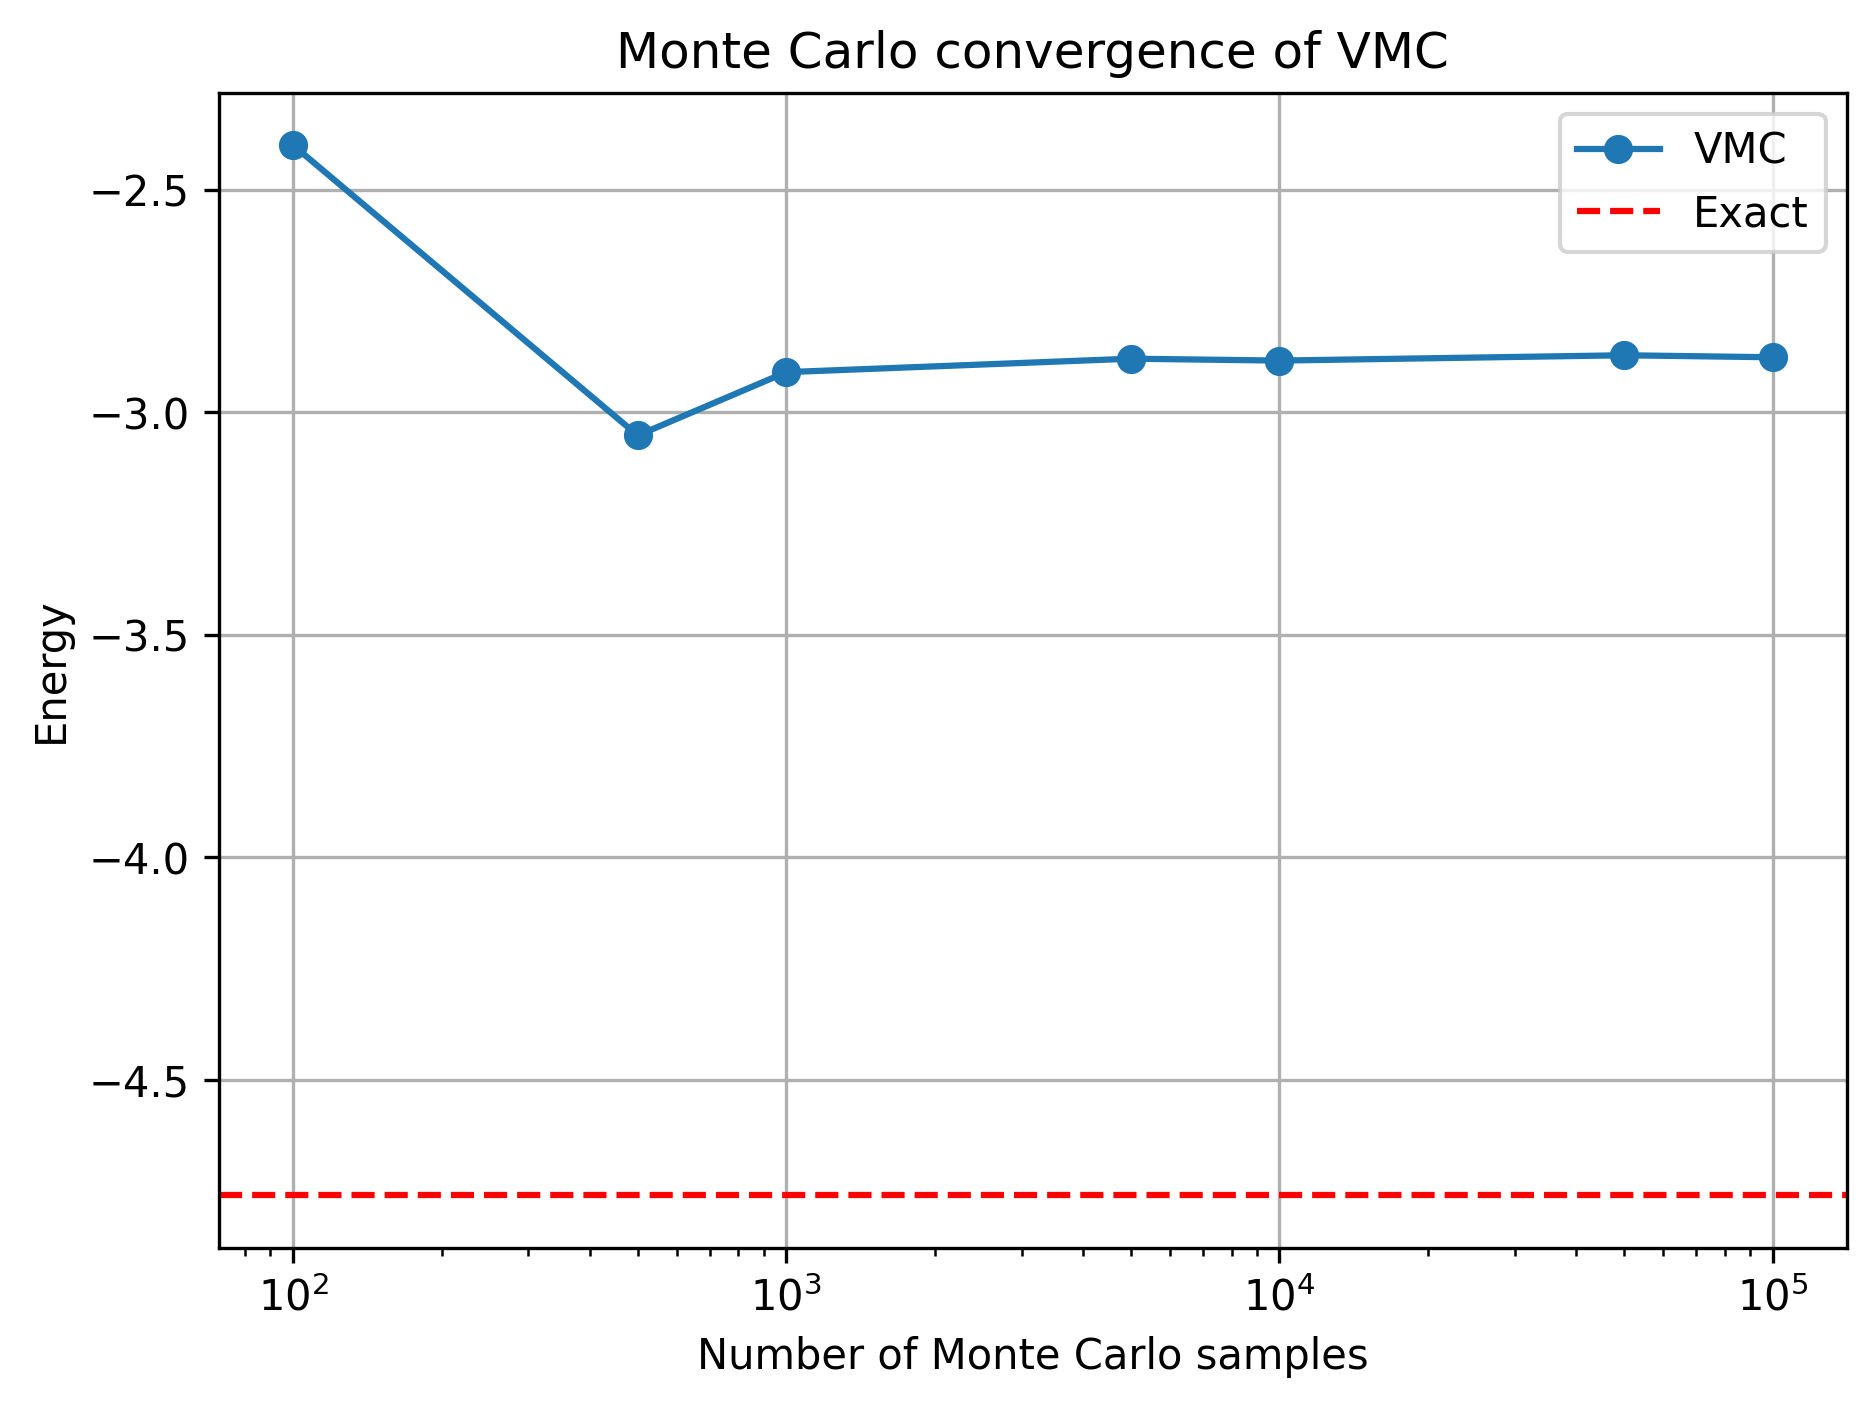
\includegraphics[width=0.6\textwidth]{../results/mc_convergence_plot.png} % 放你的实验图
		\caption{变分能量估计值随蒙特卡洛采样数的变化曲线图}
		\label{fig:2}
	\end{figure}
	如图2所示，当样本数量较少时，估计的能量表现出显著的波动，这源于随机采样的统计不确定性。随着样本量的增加，能量估计值变得越来越稳定，这表明蒙特卡洛统计误差正在逐渐减小。该收敛行为符合预期的标度关系：
	\begin{equation}
		\sigma \propto N_s^{-1/2}
	\end{equation}
	这验证了蒙特卡洛采样程序的实现是正确的，并为后续的变分优化提供了一个可靠的能量估计器。
	
	
	
	% --- 4. 遇到的问题与思考 ---
	\section{未经过优化的 RBM 初始能量计算/评估}
	我们首先评估随机初始化的受限玻尔兹曼机（RBM）态的变分能量。由于蒙特卡洛抽样的存在，估计出的能量会在一个稳定值附近波动；同时，由于模型参数保持不变，因此观察不到系统性的能量下降。
	
	\section{RBM-变分蒙特卡洛优化}
	我们采用变分能量最小化策略，利用蒙特卡洛方法估计的梯度来优化 RBM 参数。从随机初始化的 RBM 初态出发，系统能量自大约 -3.94 起开始逐渐平稳下降。最终下降到-4.40。
	在经历了 500 次优化迭代后，能量的显著降低表明神经网络量子态（NQS）成功捕捉到了横场伊辛模型的关联结构。其与精确基态能量之间残存的偏差，则归因于有限的采样噪声、受限玻尔兹曼机（RBM）有限的表达能力以及所采用的一阶梯度优化算法。分析可能由以下原因造成。
	\begin{figure}[H]
		\centering
		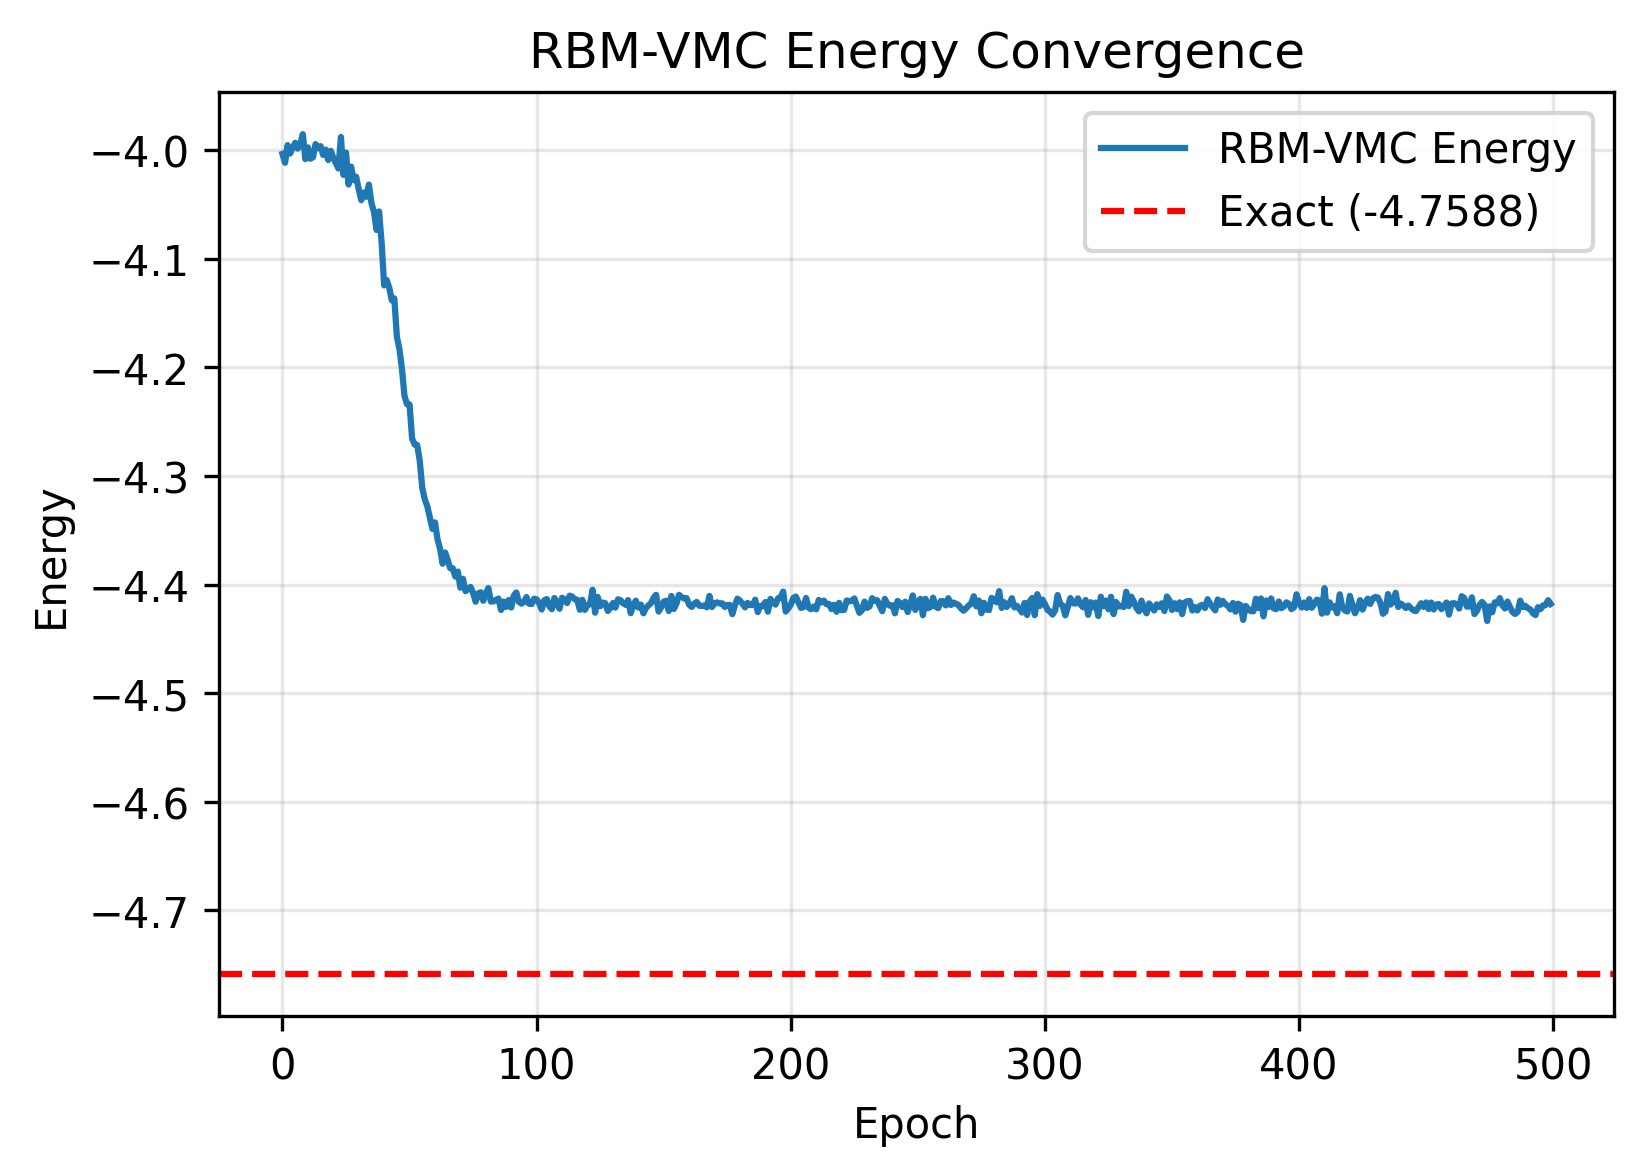
\includegraphics[width=0.6\textwidth]{../results/rbm_energy_convergence.png} % 放你的实验图
		\caption{无优化条件下能量迭代情况}
		\label{fig:3}
	\end{figure}
	
	\begin{quote}
		\begin{itemize}
			\item[原因一] RBM的容量可能不够，目前$\text{N}_\text{visible}$,$\text{N}_\text{hidden}$，可能会接近一个局部表达，可以尝试调整变大。
			
			\item[原因二] 优化算法太原始，目前的梯度下降公式是：
			\begin{equation}
				\theta_{t+1} = \theta_t - \eta \nabla E
			\end{equation}
			但是由于蒙特卡洛的噪声，容易摇摆和停在局部区域，应该尝试替换为Adam优化器与随机重整化。
			
			\item[原因三] 采样数可能偏少，因为梯度不是只有一个变量$E$，而是需要$\langle E_{\text{loc}} O_\theta \rangle$。
		\end{itemize}
	\end{quote}
	\subsection{适用于可扩展VMC的稀疏哈密顿量求值}
	在传统精确计算中，局域能量需要显式构造完整 Hamiltonian 矩阵，其计算复杂度随着系统规模呈指数增长。针对横场 Ising 模型的局域连接结构，本文实现了基于 Hamiltonian 稀疏性的局域能量计算方法，仅需遍历当前构型的有限邻接状态，将单次局域能量计算复杂度由 $O(2^N)$ 降低至 $O(N)$。其中局域的能量计算方法有：
	\begin{equation}
		Eloc​(s)=−Ji∑​si​si+1​−hi∑​ψ(s)ψ(s(i))​
	\end{equation}
	其中 $s^{(i)}$ 是把第 $i$ 个自旋翻转后的态。这样每个样本的开销从 $O(2^N)$ 降到 $O(N)$，
	而且完全不需要维护/索引整个 basis 列表（\texttt{basis.index(tuple(s))} 这一步本身也是
	$O(2^N)$ 的线性查找，非常浪费）。为了验证猜想，做了一个对比实验，看是否从全局搜索到利用伊辛模型的局限性，能优化计算时间，结果如图四所示。
	\begin{figure}[H]
		\centering
		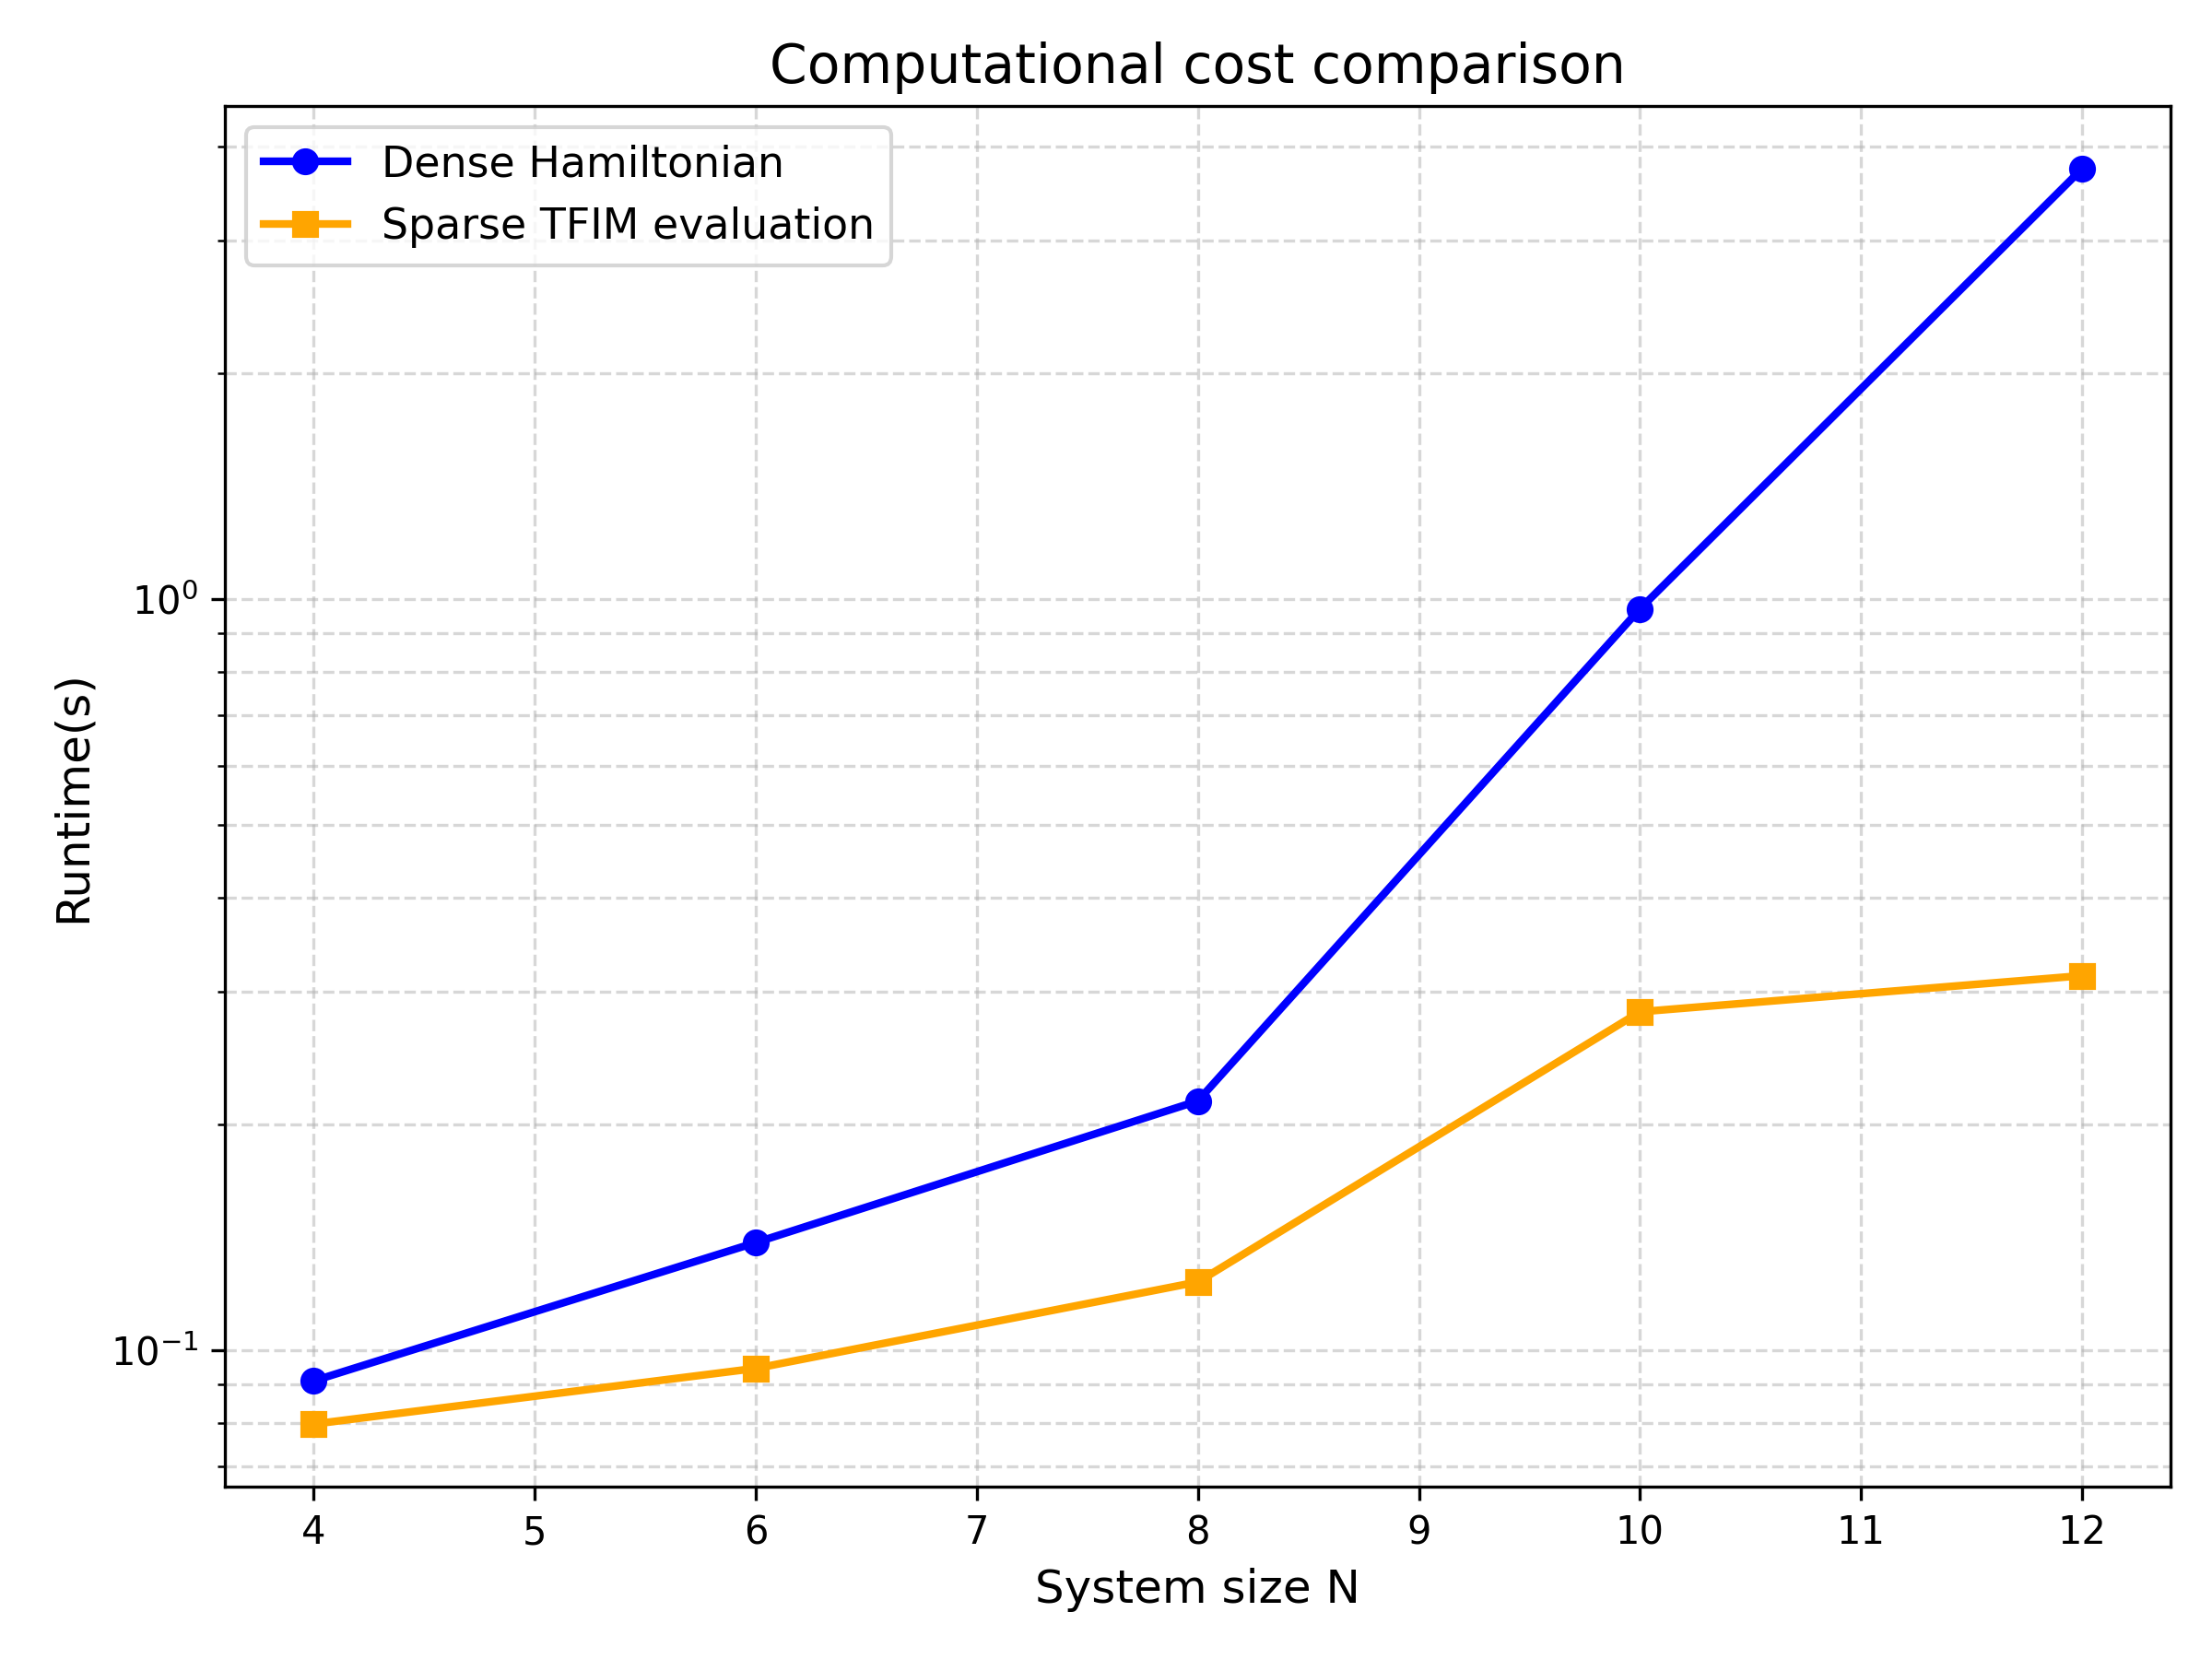
\includegraphics[width=0.6\textwidth]{../results/computational_cost_comparison.png} % 放你的实验图
		\caption{不同 Hamiltonian 计算策略的时间复杂度比较}
		\label{fig:4}
	\end{figure}
	我们验证了稀疏局部能量计算方法能准确复现稠密矩阵计算结果，同时将计算复杂度从指数级降低到线性。该优化为后续大规模神经量子态训练提供了计算基础，使得 VMC 方法能够突破小规模 Hilbert space 枚举限制。在此基础上，进一步研究更加高表达能力的神经网络波函数表示成为可能。
	\begin{figure}[H]
		\centering
		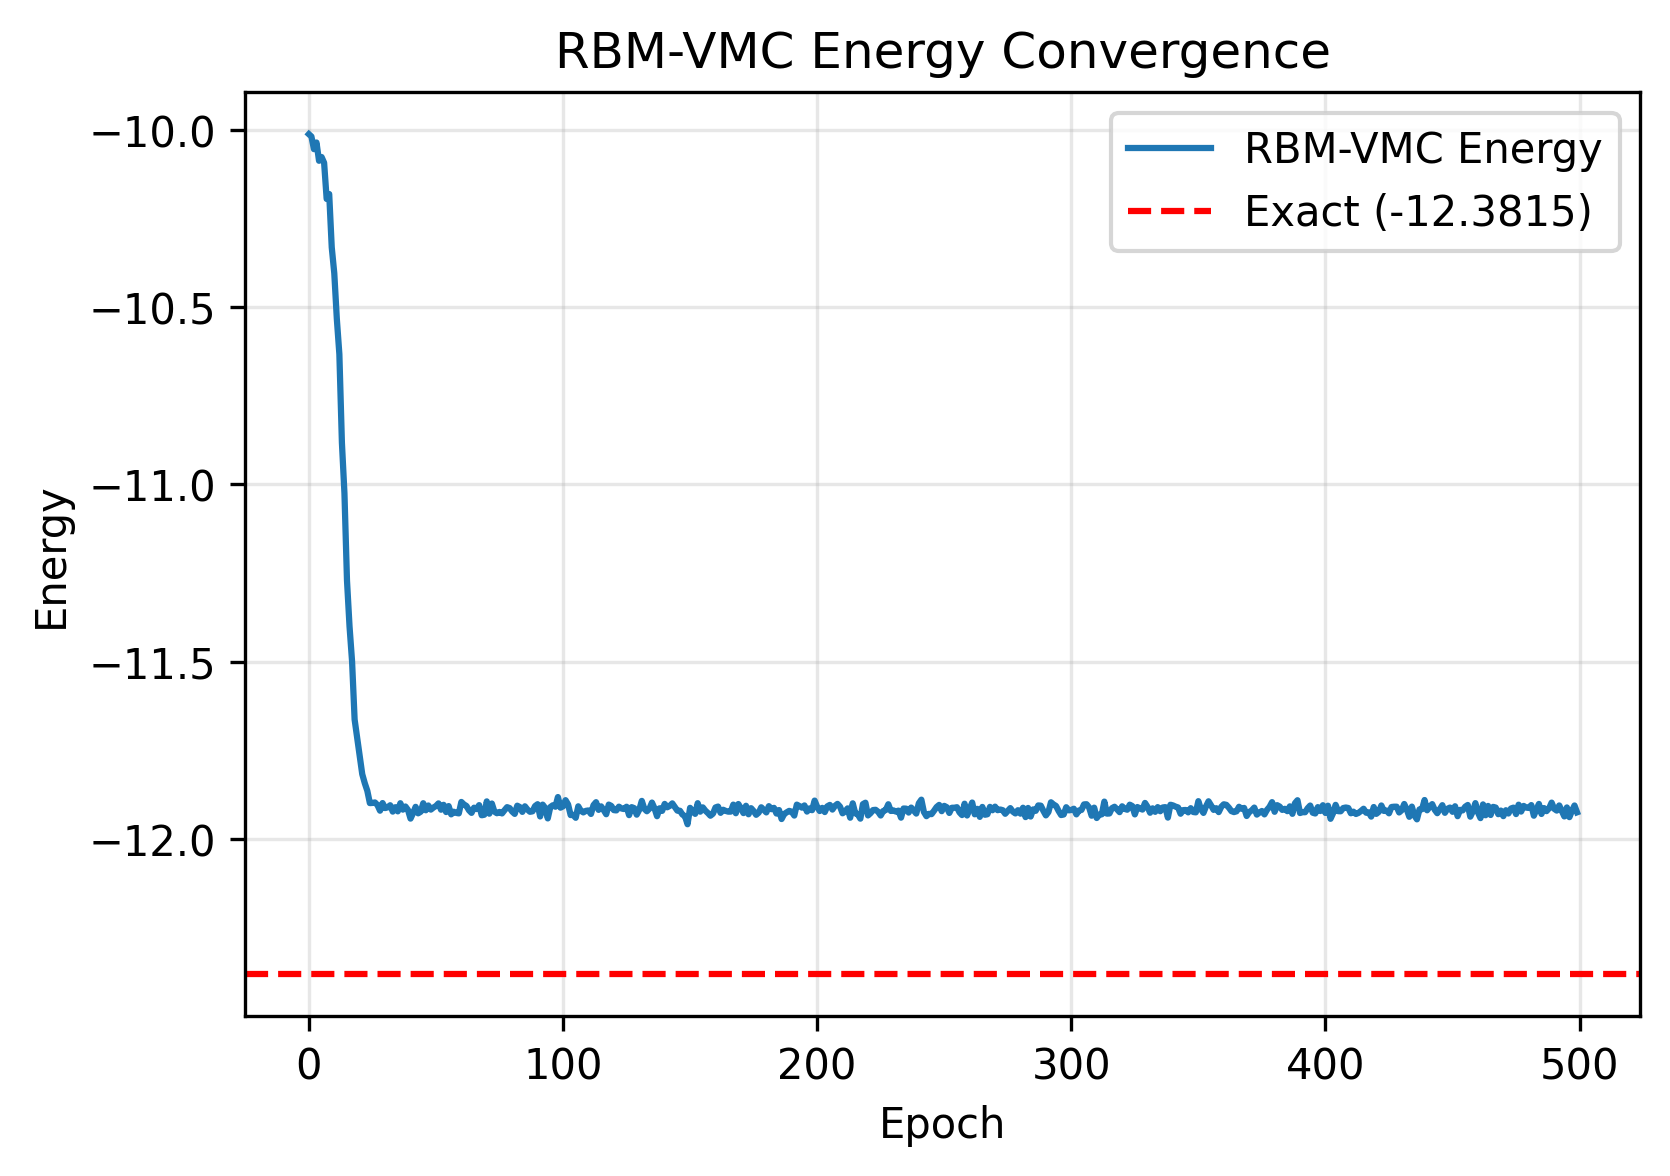
\includegraphics[width=0.6\textwidth]{../results/rbm_energy_convergence_2.png} % 放你的实验图
		\caption{$N=10$ 横场伊辛模型（TFIM）下 RBM-VMC 的能量收敛性}
		\label{fig:5}
	\end{figure}
	图5 展现了 $N=10$ 横场伊辛模型下 RBM-VMC 算法的能量收敛曲线。本实验以精确对角化（ED）得到的基态能量（$-12.3815$）作为性能基准。结果表明，变分能量在前 30 个 Epoch 内迅速下降并趋于稳定，成功达到了稳定的能量极小值，验证了模型良好的收敛性与计算效率。然而，由于浅层 RBM 表达能力的局限性，收敛后的能量（约 $-11.9$）与 ED 精确解之间仍存在微小残差（严格满足变分原理 $E_{\text{VMC}} \ge E_{\text{exact}}$），这也进一步验证了在更大系统规模下引入表达能力更强架构（如 Transformer）的必要性。
	\section{SGD与Adam模型对比分析}
	我们设计了一组实验，当$N=10,\ \text{epochs}=300,\ \text{samples}=5000,\ \text{hidden\_sizes}=[4,8,16,32,64]$时，对比两个优化器SGD与Adam的能量变化情况。
	\begin{table}[htbp]
		\centering
		\caption{不同隐层维度 $N_h$ 下 SGD 与 Adam 优化器的能量收敛值对比}
		\label{tab:sgd_vs_adam}
		\begin{tabular}{ccc}
			\toprule
			隐层维度 $N_h$ & SGD 结果 & Adam 结果 \\
			\midrule
			4  & $-11.905$ & $-11.907$ \\
			8  & $-11.907$ & $-11.906$ \\
			16 & $-11.907$ & $-11.904$ \\
			32 & $-11.900$ & $-11.900$ \\
			64 & \textcolor{red}{$-11.064$} \textsuperscript{$\dagger$} 
			& \textcolor{blue}{$-11.897$} \textsuperscript{$\ddagger$} \\
			\bottomrule
		\end{tabular}
		\vspace{0.5em}
		\begin{flushleft}
			\footnotesize
			\textsuperscript{$\dagger$} \textcolor{red}{SGD 优化崩溃，能量值显著偏高。} \\
			\textsuperscript{$\ddagger$} \textcolor{blue}{Adam 保持稳定收敛，能量正常。}
		\end{flushleft}
	\end{table}
增大隐藏层数量（4→64）、更换更稳健的优化器（SGD→Adam），均未能突破约$-11.90$的能量瓶颈，且变分原理上界条件
\[
E_{\text{VMC}} \ge E_{\text{exact}}
\]
始终被严格满足。这一结果说明能量残差主要来源于RBM架构自身的表达能力局限，而非优化过程缺陷或采样噪声干扰，这亦是本文引入Transformer架构的直接动机。
	
	% --- 5. 下一步工作计划 ---
	\section{下一步工作计划 (Next Steps)}
	\begin{itemize}
		\item [1.] 将 RBM 替换为 Transformer quantum state，并研究参数条件化量子态表示.
	\end{itemize}
	
	\vspace{2em}
	% --- 【新增】参考文献部分 ---
	% 采用 standard bibliography 环境，无需额外配置 .bib 文件，非常适合日常轻量汇报
	%\begin{thebibliography}{99}
		
	%	\bibitem{ref_classic} 
	%	作者名. 论文题目[J]. 期刊名称, 2026, 45(2): 123-130.
		
	%	\bibitem{ref_sample} 
	%	第二篇文献作者. 书籍/文章名称[M]. 出版社/期刊, 2025.
		
	%\end{thebibliography}
	
\end{document}